% ToDo: Cite DEM2016
\section{Versuchsaufbau}

\subsection{Physikalischer Aufbau}

Der schematische Aufbau eines Schüttgutsortierers kann Abbildung \ref{fig:SimAufbau} entnommen werden. Er besteht aus verschiedenen Bestandteilen: Partikel gelangen aus dem Partikelbehälter in eine Rüttelrinne. Diese sorgt für eine gleichmäßige Zuführung der Partikel in die Anlage. Nach einer weiteren, kurzen Rüttelrinne gelangen die Partikel über eine Rutsche auf das Förderband, welches mit konstanter Geschwindigkeit läuft. Das Förderband übt dabei eine Kraft auf die aufgenommenen Partikel aus, welche zu einer Veränderung der äußeren Eigenschaften der Partikel führt (z. B. Geschwindigkeit). Am Ende des Förderbandes gehen die Partikel in einen freien Flug über, um dann in einem von mehreren Auffangbehältern einsortiert zu werden (nicht sichtbar). Der Düsenbalken am Ende des Förderbandes in Kombination mit einer Flugbahnvorhersage ermöglicht es, die Flugbahn einzelner, automatisch bestimmter Partikel präzise mit Hilfe eines gezielten Druckluftstrahles zu beeinflussen. Dies erlaubt die Sortierung von Schüttgutpartikeln, indem Partikel verschiedener Beschaffenheiten in verschiedene Behälter ausgeblasen werden.

\begin{figure}[H]
    \centering
    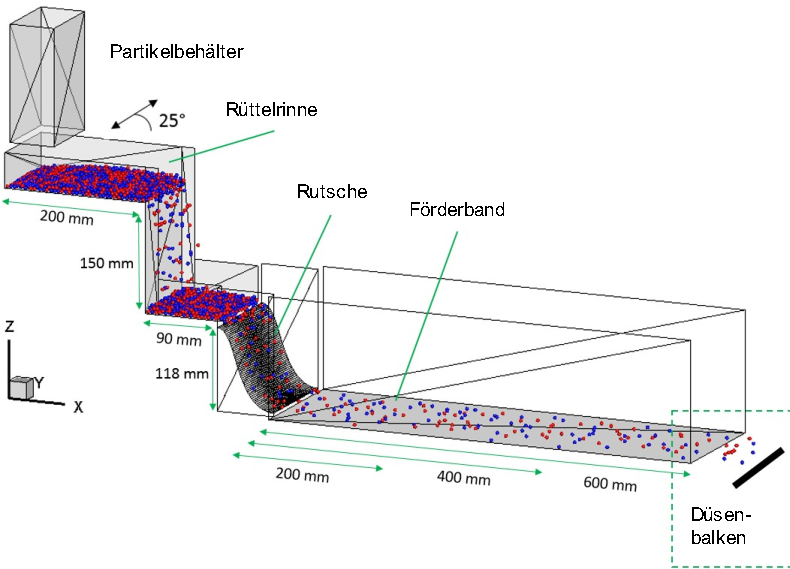
\includegraphics[width=0.7\textwidth]{pics/SimulationsAufbau.pdf}
    \caption{Schematischer Aufbau eines Schüttgutsortierers \cite{ITM07_BrunnSawo}}
    \label{fig:SimAufbau}
\end{figure}

\subsection{Kamerasystem}
Üblicherweise wird die Erkennung (Klassifikation) der Partikel, welche für die Sortierung benötigt wird, mit Hilfe einer am Ende des Förderbandes positionierten Zeilenkamera durchgeführt. Eine Zeilenkamera weißt lediglich eine Zeile lichtempfindlicher Zellen auf, und kann damit kein zweidimensionales Bild liefern (TODO stimmt so nicht ganz, man kann auch mit Zeilenkameras ein 2D-Bild vorbeifliegender Objekte rekonstruieren). Damit ermöglicht sie die Klassifikation der Partikel ausschließlich auf Basis optischer Merkmale und nicht zum Beispiel anhand des Bewegungsverlaufs.

Im vorliegenden Fall wird die Zeilenkamera durch eine Flächenkamera ergänzt, welche ein zweidimensionales Bild liefert. Das Bild umfasst den hinteren Abschnitt des Bandes mit einer Frequenz zwischen 100 und 250 Hz (siehe Abbildung \ref{fig:SimKameras}). Durch Methoden der digitalen Bildverarbeitung kann auf diese Weise ein Tracking der Partikel über die Zeit durchgeführt werden. Dies ermöglicht die Bestimmung des Bewegungsprofils jedes einzelnen Partikels, welches wiederum für eine präzisere Flugbahnvorhersage genutzt werden kann. Diese wiederum kann zum gezielteren Ausblasen einzelner Partikel genutzt werden und senkt somit die Gesamtfehlerrate des Sortierers. Der Gesamtaufbau eines um eine Flächenkamera erweiterten Systems kann Abbildung \ref{fig:SimGesamt} entnommen werden.

Die durch das Tracking extrahierten Bewegungsprofile sollen im Zuge dieser Arbeit nicht mehr nur zur Flugbahnvorhersage, sondern wie bereits in Kapitel \ref{sec:Motivation} beschrieben an Stelle der bisher verwenden optischen Daten der Zeilenkamera auch zur Klassifikation der Partikel eingesetzt werden.

\begin{figure}[H]
    \centering
    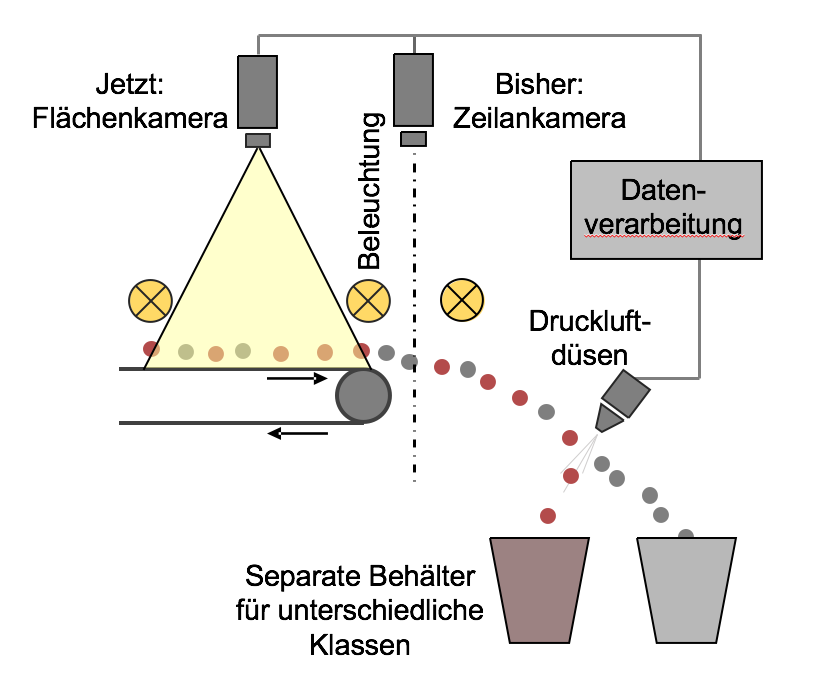
\includegraphics[width=0.4\textwidth]{pics/Kameras.png}
    \caption{Positionierung von Zeilen- und Flächenkamera}
    \label{fig:SimKameras}
\end{figure}


\begin{figure}[H]
    \centering
    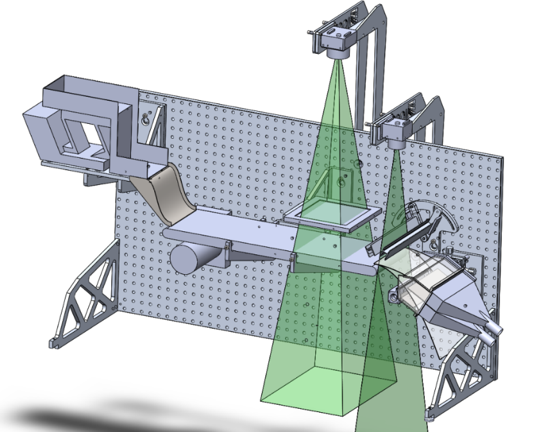
\includegraphics[width=0.7\textwidth]{pics/Anlage1.png}
    \caption{Aufbau des Gesamtsystems am Beispiel des TableSort-2-Schüttgutsortierers \cite{TableSort}}
    \label{fig:SimGesamt}
\end{figure}

\subsection{Vorliegende Daten}
Die dieser Arbeit zugrunde liegenden Beispieldaten stammen aus zwei verschiedenen Quellen: Zum Einen aus Realdaten, die mit Hilfe eines existierenden Schüttgutsortierers erhoben wurden, und zum anderen aus einer eigens für diesen Anwendungsfall durch die UNI BOCHUM durchgeführten Simulation, welche einen Schüttgutsortierer und verschiedene Arten von Partikeln simuliert. Die Datenmenge der verfügbaren Simulationsdaten ist dabei wesentlich größer als die Menge verfügbarer Realdaten. Beide Datenquellen werden im Folgenden detailliert beschrieben. % ToDo: Ref

\subsubsection{Simulation} \label{DataSimulation}

Die durch die UNI BOCHUM durchgeführte Simulation beschreibt exakt den in Abbildung \ref{fig:SimAufbau} illustrierten Schüttgutsortierer. Alle aus der Simulation gewonnenen Datensätze weisen dabei sehr ähnliche Randbedingungen auf: Jeder Datensatz erfasst verschiedene physikalische Größen der Partikel mit exakt 1000 Hz. Dabei werden Partikel nicht nur, wie in realen Anwendungsfällen, auf dem durch die Kamera beobachteten Abschnitt des Bandes, sondern über die gesamte Anlage hinweg aufgenommen. Folgende physikalische Größen werden dabei erhoben:

\begin{description}
\item[Position] Position des Partikels in x, y und z-Richtung
\item[Momentane Geschwindigkeit] Momentane Geschwindigkeit des Partikels in x, y und z-Richtung
\item[Kräfte] Auf das Partikel wirkende Kräfte in x, y und z-Richtung
\item[Durchmesser] Durchmesser des Partikels
\item[Masse] Masse des Partikels
\item[ID] Identifier des Partikels, für Zuordnung von Datenpunkt zu Partikel
\item[Farbe] Simulierte Farbe des Partikels
\item[Art] Klasse, der das Partikel zugeordnet wird
\end{description}

Zum Erreichen des in Kapitel \ref{sec:Goal} beschriebenen Ziels, möglichst wenige, realistische Annahmen zu treffen, wurde von Beginn an auf die Nutzung einiger nur in der Simulation zur Verfügung stehenden Daten verzichtet. Dabei handelt es sich hauptsächlich um physikalische Größen, die mit der verwendeten Sensorik in Kombination mit dem Tracking nicht messbar sind. Beispiel für nicht verwendbare Daten sind z.B. Kräfte (können nicht mit einer Flächenkamera gemessen werden), Durchmesser (ebenfalls mit einer Flächenkamera nicht messbar, würde ein 3D-Modell jedes Partikels voraussetzen) sowie Masse (würde eine Waage benötigen). Auch die Geschwindigkeiten werden nicht verwendet, da eine Flächenkamera diese nicht direkt extrahieren kann. Ebenfalls verworfen wurde außerdem die z-Position aller Partikel, da für die Erfassung der z-Koordinate der Einsatz einer Stereokamera nötig wäre. Die IDs, Farben und Art der Partikel wurden lediglich als Metadaten verwendet. Darüber hinaus wurden nur Datenpunkte betrachtet, die in der xy-Ebene im Bereich des Bandes liegen, da ein Realsystem keine Messwerte im Bereich der Rüttelrinnen oder Rutsche liefert. Abschließend wurden vier von fünf Datenpunkten verworfen, mit dem Ziel eine Messfrequenz von 250 Hz zu simulieren - der maximalen, an realen Anlagen mit der beschriebenen Sensorik erreichbaren Frequenz.

Zur Verfügung standen vier Datensätze von Partikel unterschiedlicher Eigenschaften: Quader, Zylinder und zwei Arten von Kugeln mit unterschiedlichen Dichten. Zusätzlich wurde die Kombination von Kugeln und Quadern simuliert. Die Datensätze enthalten jeweils eine Aufnahme der Partikel über 20s, wobei jeweils zwischen 4000 und 4500 eindeutige Partikel beobachtet wurden --- in Summe standen also die Beobachtungen von ca. 17000 Partikeln zur Verfügung. Die schnelle Generierung neuer Simulationsdaten war jedoch nicht möglich, da die Simulation selbst auf einem Großrechner Laufzeiten in der Größenordnung von einer Woche aufweist --- für Datensätze ähnlicher Größe. % ToDo: correct number

\subsubsection{Realdaten}

Die zweite verfügbare Datenquelle umfasst die Ergebnisse des Trackings, das auf Bilddaten aus einer realen Anlage (TableSort 2, siehe Abbildung \ref{fig:SimGesamt}) angewendet wurde. Bei der einzigen erfassten physikalische Größe handelt es sich um die Position der Partikel auf der xy-Ebene zu verschiedenen Zeitpunkten. Alle anderen Daten, wie z. B. die Geschwindigkeit, müssen aus den Positionsdaten abgeleitet werden. Das Tracking wurde auf vier verschiedene Partikelarten angewendet, welche weniger abstrakt sind als die in der Simulation verwendeten Partikelarten: Kugeln, Halbkugeln, Wachsperlen und Wattekugeln. Für jede Partikelart stehen zwei Datensätze zur Verfügung, welche jeweils Daten für 45--130 Partikel erhalten. Für jeden Partikel wurden dabei zwischen zwei und 25 Samples erfasst.

\subsubsection{Datenmenge}

Alles in allem steht, in Relation zu realistischen Anwendungsfällen, nur eine sehr kleine Datenmenge zur Verfügung. Die Simulationsdaten enthalten pro Datensatz jeweils nur einen 20-sekündigen Ausschnitt, welcher nur zu Beginn eine größere Menge an Partikeln umfasst. Die Realdatensätze enthalten eine noch weitaus geringere Menge verwertbarer Daten, und besitzen daher verglichen mit den Simulationsdaten kaum Aussagekraft. Es ist davon auszugehen, dass eine reale Anlage in kürzester Zeit weitaus größere Datenmengen liefern kann.

% \fbox{\parbox{\textwidth}{
% \noindent\textbf{Inhalt}
% \begin{itemize}
% \item Simulierte Datensätze
%         \begin{itemize}
%             \item Einzelne Datensätze (Kugeln, Kugeln mit andere Dichte, Zylinder, Quader)
%             \item Gemischte Datensätze
%         \end{itemize}
%     \item Realdaten
% \end{itemize}
% }}
